\documentclass[crop, tikz]{standalone}

\usepackage[utf8]{inputenc}
% 'crop' is the default for v1.0, before it was 'preview'
%\usetikzlibrary{...}% tikz package already loaded by 'tikz' option

\usetikzlibrary{arrows}
\usetikzlibrary{decorations.markings}
\usetikzlibrary{patterns}
\usetikzlibrary{calc}

%hexagon drawing variables
\def\ly{0.866025} %sin(pi/3) = sqrt(3)/2
\def\lx{0.5} %cos(pi/3) = 0.5
\def\hexSize{5} %size of the hexagon that'll be the extent of the fibre cross section
\def\coreSize{0.2} %size of hollow cores
\def\coreSep{0.5} %separation between core CENTRES HORIZONTALLY
\def\coreSepHeight{0.4464} %separation between core CENTRES VERTICALLY

\newcommand{\hexagon}[4]{
\begin{scope}[shift={#2}]
	\draw[#3, fill=#4] (-#1*\lx, #1*\ly) -- (#1*\lx, #1*\ly) -- (#1,0) -- (#1*\lx, -#1*\ly) -- (-#1*\lx, -#1*\ly) -- (-#1,0) -- cycle;
\end{scope}
} %\hexagon{centre-to-corner-length}{shift (x,y)}{line spec}{fill colour} [none is allowed for fillcolour]

\begin{document}
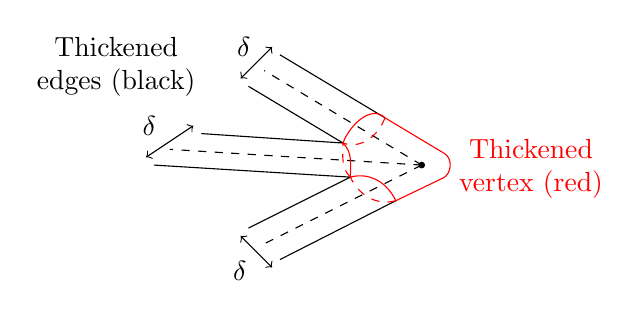
\begin{tikzpicture}[]
	
	% save coordinates for later
	\coordinate (v0) at (0,0);
	\coordinate (v1) at (-2,1.2);			\coordinate (v1bar) at (-7/15,3/5);
	\coordinate (v2) at (-3.2,0.2);
	\coordinate (v3) at (-2,-1);				\coordinate (v3bar) at (-28/85,-77/170);
	\coordinate (v12) at (-1,7/25);
	\coordinate (v23) at (-77/85,-13/85);

	% draw the junction's skeleton first...
	\filldraw[black] (v0) circle (1pt);
	% draw edges coming out of the vertex, and one connecting vertex
	\draw[dashed] (v0) -- (v1);
	\draw[dashed] (v0) -- (v2);
	\draw[dashed] (v0) -- (v3);

	% draw tubes...
	\draw (-1.8,1.4) -- (v1bar);
	\draw[red] (v1bar) -- (16/55,8/55) to[out=-30.963756532, in=26.565051177] (3/11,-9/55) -- (v3bar);
	\draw (v3bar) -- (-1.8,-1.2);
	\draw (-2.8,0.4) -- (v12) -- (-2.2,1.0);
	\draw (-3.4,0.0) -- (v23) -- (-2.2,-0.8);

	%vertex region in red
	\draw[red] (v12) to[out=90-20, in=90+45] (v1bar);
	\draw[red, dashed] (v1bar) to[out=270-20, in=-20] (v12);
	\draw[red] (v12) to[out=-90+45, in=90] (v23);
	\draw[red, dashed] (v23) to[out=135, in=270] (v12);
	\draw[red] (v23) to[out=15, in=90+25] (v3bar);
	\draw[red, dashed] (v3bar) to[out=180+15, in=-65] (v23);

	% nodes with labels
	\node[anchor=west, align=center, red] at (0.35,-0.05) {Thickened \\ vertex (red)};
	\node[anchor=south east, align=center] at (-2.75,0.75) {Thickened \\ edges (black)};

	% indicate width of tubes
	\draw[<->] (-2.2-0.1,1.0+0.1) -- (-1.8-0.1,1.4+0.1);
	\node[anchor=south east] at (-2-0.05,1.2+0.05) {$\delta$};
	\draw[<->] (-3.4-0.1,0.0+0.1) -- (-2.8-0.1,0.4+0.1);
	\node[anchor=south east] at (-3.2-0.05,0.2+0.05) {$\delta$};	
	\draw[<->] (-2.2-0.1,-0.8-0.1) -- (-1.8-0.1,-1.2-0.1);
	\node[anchor=north east] at (-2-0.1,-1-0.1) {$\delta$};

\end{tikzpicture}
\end{document}